\documentclass[a4paper,11pt, uplatex,openany]{jsbook}

%%%% Packages
%\usepackage{fancyhdr}
\usepackage{thesis2017} 

%
%% 以下, 必要ないものは消してください. 
%\usepackage{fancyhdr}
\usepackage{layout} % 第3章中の \layout のためだけなので, 論文執筆には不要. 
\usepackage[dvipdfmx,hidelinks]{hyperref} % 目次をクリックするとそのページに飛ぶ.
\usepackage{pxjahyper} % hyperrefを使った時に文字化けする場合は使う.
\usepackage{amsmath} % 数式扱うなら必須.
\usepackage{ascmac} % 文章の枠囲み. 論文では不要だと思う.  
\usepackage[dvipdfmx]{xcolor} % 文字に色をつける. これも不要. 
\usepackage[dvipdfmx]{graphicx} % 図の挿入に必要. 
\usepackage[skip=5pt]{caption} % あった方がいい. 
\captionsetup{labelfont=bf} % あった方がいい. 
\usepackage[
  labelformat=simple, 
  list=true, 
  listformat=simple]{subcaption} % 図3.2(a)的なことをする場合は必要
  \renewcommand\thesubfigure{(\alph{subfigure})} % 図3.2(a)的なことをする場合は必要
 

%%%% Settings
\bibliographystyle{junsrt}

%%%% \def: Definitions
\def\diff{\mathrm{d}}
\def\BibTeX{B{\small IB}\TeX}

%通し番号の参照
\def\figname{Fig.~}
\def\tabname{Table~}
\newcommand{\eqnname}{式~}
\renewcommand{\figurename}{Fig.~}
\renewcommand{\tablename}{Table~}

%%%%%%%% Document
\begin{document}

%
%前書き
\frontmatter
\clearpage
% タイトルページ
\begin{titlepage}
\centering
\vspace*{40truept}
{\Large 平成30年度 修士論文} \\ % 年度
\vspace{40truept} 
 {\Large 題目} \\
 \vspace{10truept} 
{\LARGE \textbf{圧力センサを用いた油圧アクチュエータの力制御}}\\ % タイトル
\vspace{10truept}
%{\Large --- サブタイトル ---}\\ % サブタイトル. なければコメントアウト
\vspace{120truept}
{\Large 指導教員}\\ %
 \vspace{10truept} 
{\Large 石川 将人 教授\\南 裕樹}\\ % 指導教員
\vspace{60truept}
{\Large 大阪大学大学院 工学研究科 機械工学専攻}\\ % 学科
 \vspace{10truept} 
{\Large 学籍番号 28E17076}\\ % 学籍番号
\vspace{20truept}
{\LARGE 吉田 侑史}\\ % 著者
\vspace{80truept}
{\Large 2016年2月7日} % 提出日
\end{titlepage}
\cleardoublepage
% アブストラクト
\chapter*{\huge 概要}
\vskip2\Cvs

hogehoge~


\section*{\huge Abstract}
\vskip2\Cvs
This paper discusses ...
%
%


\newpage

%目次
\tableofcontents   %目次
\thispagestyle{plain}
%\newpage
\listoffigures %図目次 図が少なければいらないかも
%\newpage
\listoftables %表目次 表が少なければいらないかも
%\newpage

 %タイトル・概要・目次など

%本文
\mainmatter
%\chapter{緒言}

\section{研究背景}
油圧アクチュエータは電動アクチュエータと比べ,外力に対する耐衝撃性・質量出力比・最大出力の大きさ・設計の自由度の高さなどに優れており,現在においても使われる分野は多い.
特に建設機械(耐衝撃性や最大出力)や航空機(質量出力比)などの分野では欠かせないものとなっている.
一方で,油漏れを防ぐためのシーリングによる摩擦や,油自身の圧縮性・温度依存性・発火性などの構造や性質に起因する制御性能の低さ,そして電動アクチュエータの高性能化により,現在では制御性能に優れる電動のものが広く使われている.

しかし,電動と油圧を組み合わせた電気油圧式アクチュエータの登場や,計算機能力および制御技術の向上により,特にロボティクスの分野において駆動力として油圧アクチュエータが見直されてきている\cite{feng2014optimization,kuindersma2016optimization,玄相昊2015招待講演}.
油圧アクチュエータが用いられている例の一つに\figname\ref{fig:PA-2000}に示す6軸油圧マニピュレータPA-2000\cite{IRID}があり,これが本研究において取り扱う対象である.

PA-2000は福島第一原子力発電所の廃炉に向けて燃料デブリを取り出すために,国際原子炉開発機構(IRID)および三菱重工株式会社により開発試作されているマニピュレータである\cite{河西賢一2018福島第一原子力発電所燃料デブリ横取り出しに向けたロボット開発}.
狭い通路\footnote{CRD交換用開口を通過する.そのため,PA-2000では外形寸法が\SI{700}{mm}$\times$\SI{920}{mm}に抑えられている.}を通過すること,デブリに対する加工反力に耐えることなどの条件を満たすために,質量出力比に優れる油圧アクチュエータが採用されている.
燃料デブリ取り出しは原子炉内という高放射線下で人が立ち入れない環境で行われ,安全に作業を進めるためには,マニピュレータ先端の位置および力を制御する必要がある.
本研究ではこのうち,手先が対象物に接触している状態において発生させる力を制御することに取り組む.

力を制御するにあたり,手先にかかる力を測定してフィードバックを行う必要があるが,力センサなどを用いて直接測定するのではなく,シリンダに取り付けた圧力センサなどを用いて手先の力を推定する手法を開発する.
力センサを用いないことで,マニピュレータ全体の省線化が図れるとともに,複数種類利用することが想定される先端ツールの設計簡略化が期待される.
また,圧力をフィードバックすることにより,マニピュレータ先端が対象物体に触れたときの姿勢に依らず力を推定できることが期待される.

圧力から力を推定する手法は,佐藤ら\cite{佐藤有香理2015油圧ショベルにおけるバケット先端の負荷力推定}がショベルにおいてなぞり作業時の負荷推定を行い,岡田ら\cite{岡田大貴2016多自由度油圧駆動ロボットのシリンダ圧に基づく手先負荷力推定,岡田大貴2017多自由度油圧駆動ロボットのシリンダ圧に基づく手先負荷力推定による力覚フィードバック}は建設機械ベースのロボットにおいて力覚フィードバックを行っている.
これらの研究ではシリンダから発生する力は圧力と受圧面積から求め,摩擦については触れられていない.
本研究では,システム同定を活用することにより摩擦の影響も含めたモデルを得ることで,より現実に近いシリンダ出力を推定する.
さらに,推定した出力をもとに,力制御系の設計を行う.

\begin{figure}[t]
    \centering
        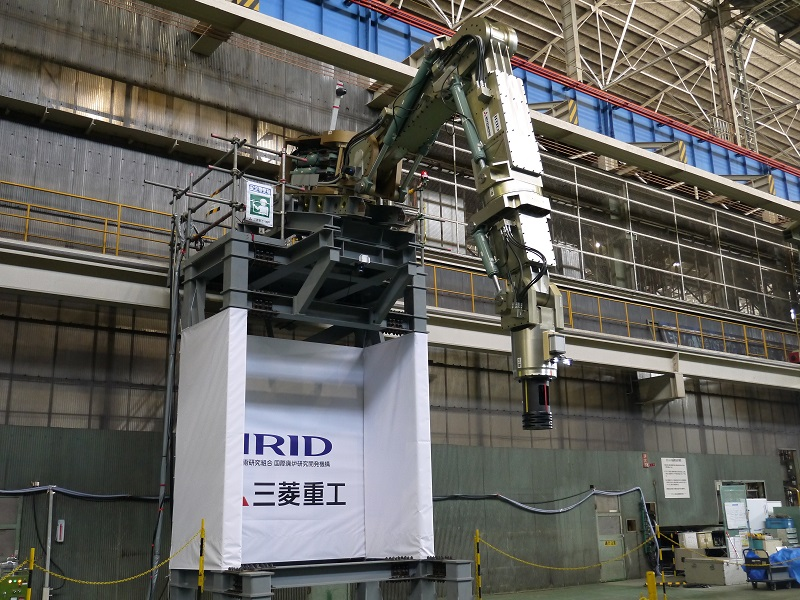
\includegraphics[keepaspectratio, width = .8\linewidth]{contents/緒言/figure/PA-2000.jpg}
        \caption{6-axis Hydraulic Manipulator: PA-2000}
        \label{fig:PA-2000}
\end{figure}

\section{力制御に向けたアプローチ}
力制御に向けたアプローチの概要を\figname\ref{fig:approach_thiswork}に示す.
いきなり6軸油圧マニピュレータで試験を行うのではなく,はじめに油圧シリンダ単体を扱う.
油圧シリンダを対象として力を推定する手法の構築および推定した力を用いたシリンダの力制御を行う.
その後,構築した手法を実験室レベルでORION-7Pへ適用し,最終的にPA-2000への適用を目指す.
ORION-7PはPA-2000と同じ関節配置を持つ油圧マニピュレータである.
本研究では最初の段階である油圧シリンダ単体を対象としてシステム同定を活用した力の推定および力制御を行う.

\begin{figure}[t]
    \centering
        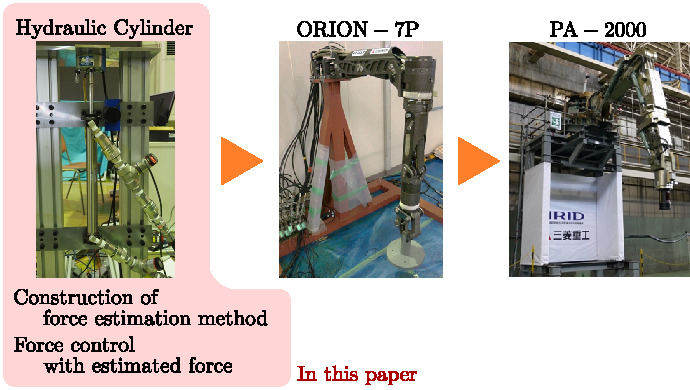
\includegraphics[keepaspectratio, scale=1.0]{contents/緒言/figure/approach_thiswork.pdf}
        \caption{Approach in this work}
        \label{fig:approach_thiswork}
\end{figure}

\section{油圧システムの特徴と関連研究}
本節では,油圧システムの特徴について述べ,油圧アクチュエータ制御の関連研究について紹介する.
\subsection{油圧システムの特徴}

油圧システムの駆動における基本原理はパスカルの原理\cite{PascalsLaw}であり,圧力発生源および圧力を伝える媒体があればアクチュエータを作動させることが可能である.
そのため,電動機の登場以前より重要な駆動力として扱われてきた.
油圧システムの利点を以下に示す\cite{jelali2012hydraulic,不二越ハイドロニクスチーム199305}.
\begin{itemize}
    \item 出力重量比(出力密度)が大きい.
    \item 最大出力が大きく,無段階で出力・速度を設定可能.
    \begin{itemize}
        \item 出力は受圧面積と圧力で決まるため,これらを変えることで出力および動作速度を設定することが可能である.
    \end{itemize}
    \item 外部からの衝撃に頑健であり,過負荷に対する保護が容易である.
    \begin{itemize}
        \item ギヤなどのかみ合わせ部品がなく,衝撃を面で受けるため耐衝撃性が高い.また,一定以上の圧力を逃す構造にすることで過負荷に対して装置本体を守ることができる.
    \end{itemize}
    \item 設計の自由度が高い.
    \begin{itemize}
        \item ホースなどが通るスペースさえあれば,圧力供給源とアクチュエータを離れたところに配置することが可能である.
    \end{itemize}
\end{itemize}

一方,欠点も存在し,その代表的なものを以下に示す.
\begin{itemize}
    \item シーリングが必須であり,それによる摩擦が存在する.
    \item 油の圧縮性や温度依存性がある.
    \item 油への異物混入に弱い.
    \item 油漏れのさいに火災の恐れがある.
\end{itemize}
摩擦や圧縮性などは,スティックスリップなどの非線形性をもたらしており,制御を難しくする要因となっている\cite{松崎淳1962直動形油圧駆動機構におけるスティックスリップ,de1995new}.


\subsection{油圧制御の関連研究}
油圧アクチュエータ制御にについて,モデル化を含め位置制御および力制御において様々な手法の適用・提案がされている.
油圧システムの同定はバルブへの指令電圧を入力,位置を出力としたものについていくつか行われており,Lingらは線形システムとみなしての同定を行い,3次の離散システムでモデル化できることを示している\cite{ling2012system}.前島らは,第一原理に基づくモデルおよび各パラメータの同定\cite{前島祐三2011,前島祐三2014}行っている.
Zulfmanらは,同定を行ったモデルに対しファジィ制御を適用し,位置制御の改善をしている\cite{zheng2009application}.

位置制御においては摩擦補償の適用が行われている\cite{jianyong2012robust,rahmat2011modeling,lischinsky1999friction}.
特に,Rahmatらは摩擦と油の内部漏れを統合して扱い,これらを補償することで性能向上を図っている\cite{rahmat2011modeling}.
また,力制御については,AlleyneらやKoivumakiらの研究があるが,位置制御と比べて数が少ないのが現状である\cite{Alleyne,koivumaki2015stability}.
%\subsubsection{油圧アクチュエータ}
%\subsubsection{油圧機械(ロボット,建設機械など)}



\section{本論文の構成}
本論文の構成は次のようになる.
\begin{itemize}
    \item [\ref{sec:FundamentalEquation}章]第一原理に基づいたシステムのモデルの記述をする.これはJelaliらの方法\cite{jelali2012hydraulic}に基づき行う.
    \item [\ref{sec:SystemIdentification}章]油圧システムのシステム同定を行い,力推定の準備をする.
    \item [\ref{sec:ForceControl}章]力制御を行う.
    力制御にあたってはPID制御やI-PD制御,$H_\infty$制御を適用し,比較を行う.
    \item [\ref{sec:IntegrationControl}章] 位置制御と力制御を組み合わせた制御を行う.また,コンプライアンス制御の適用も試みる.
\end{itemize}

\chapter{基礎方程式}
本章では油圧システムについてのモデリングの導出を行う.
対象とする油圧システムの模式図は図で表され,4ポートサーボバルブと片ロッドシリンダが接続されているものとなる.
このサーボバルブとシリンダについてJalaliら\cite{jelali2012hydraulic} に従いながら第一原理に基づき基礎方程式の記述を行う.
\begin{figure}[t]
    \centering
        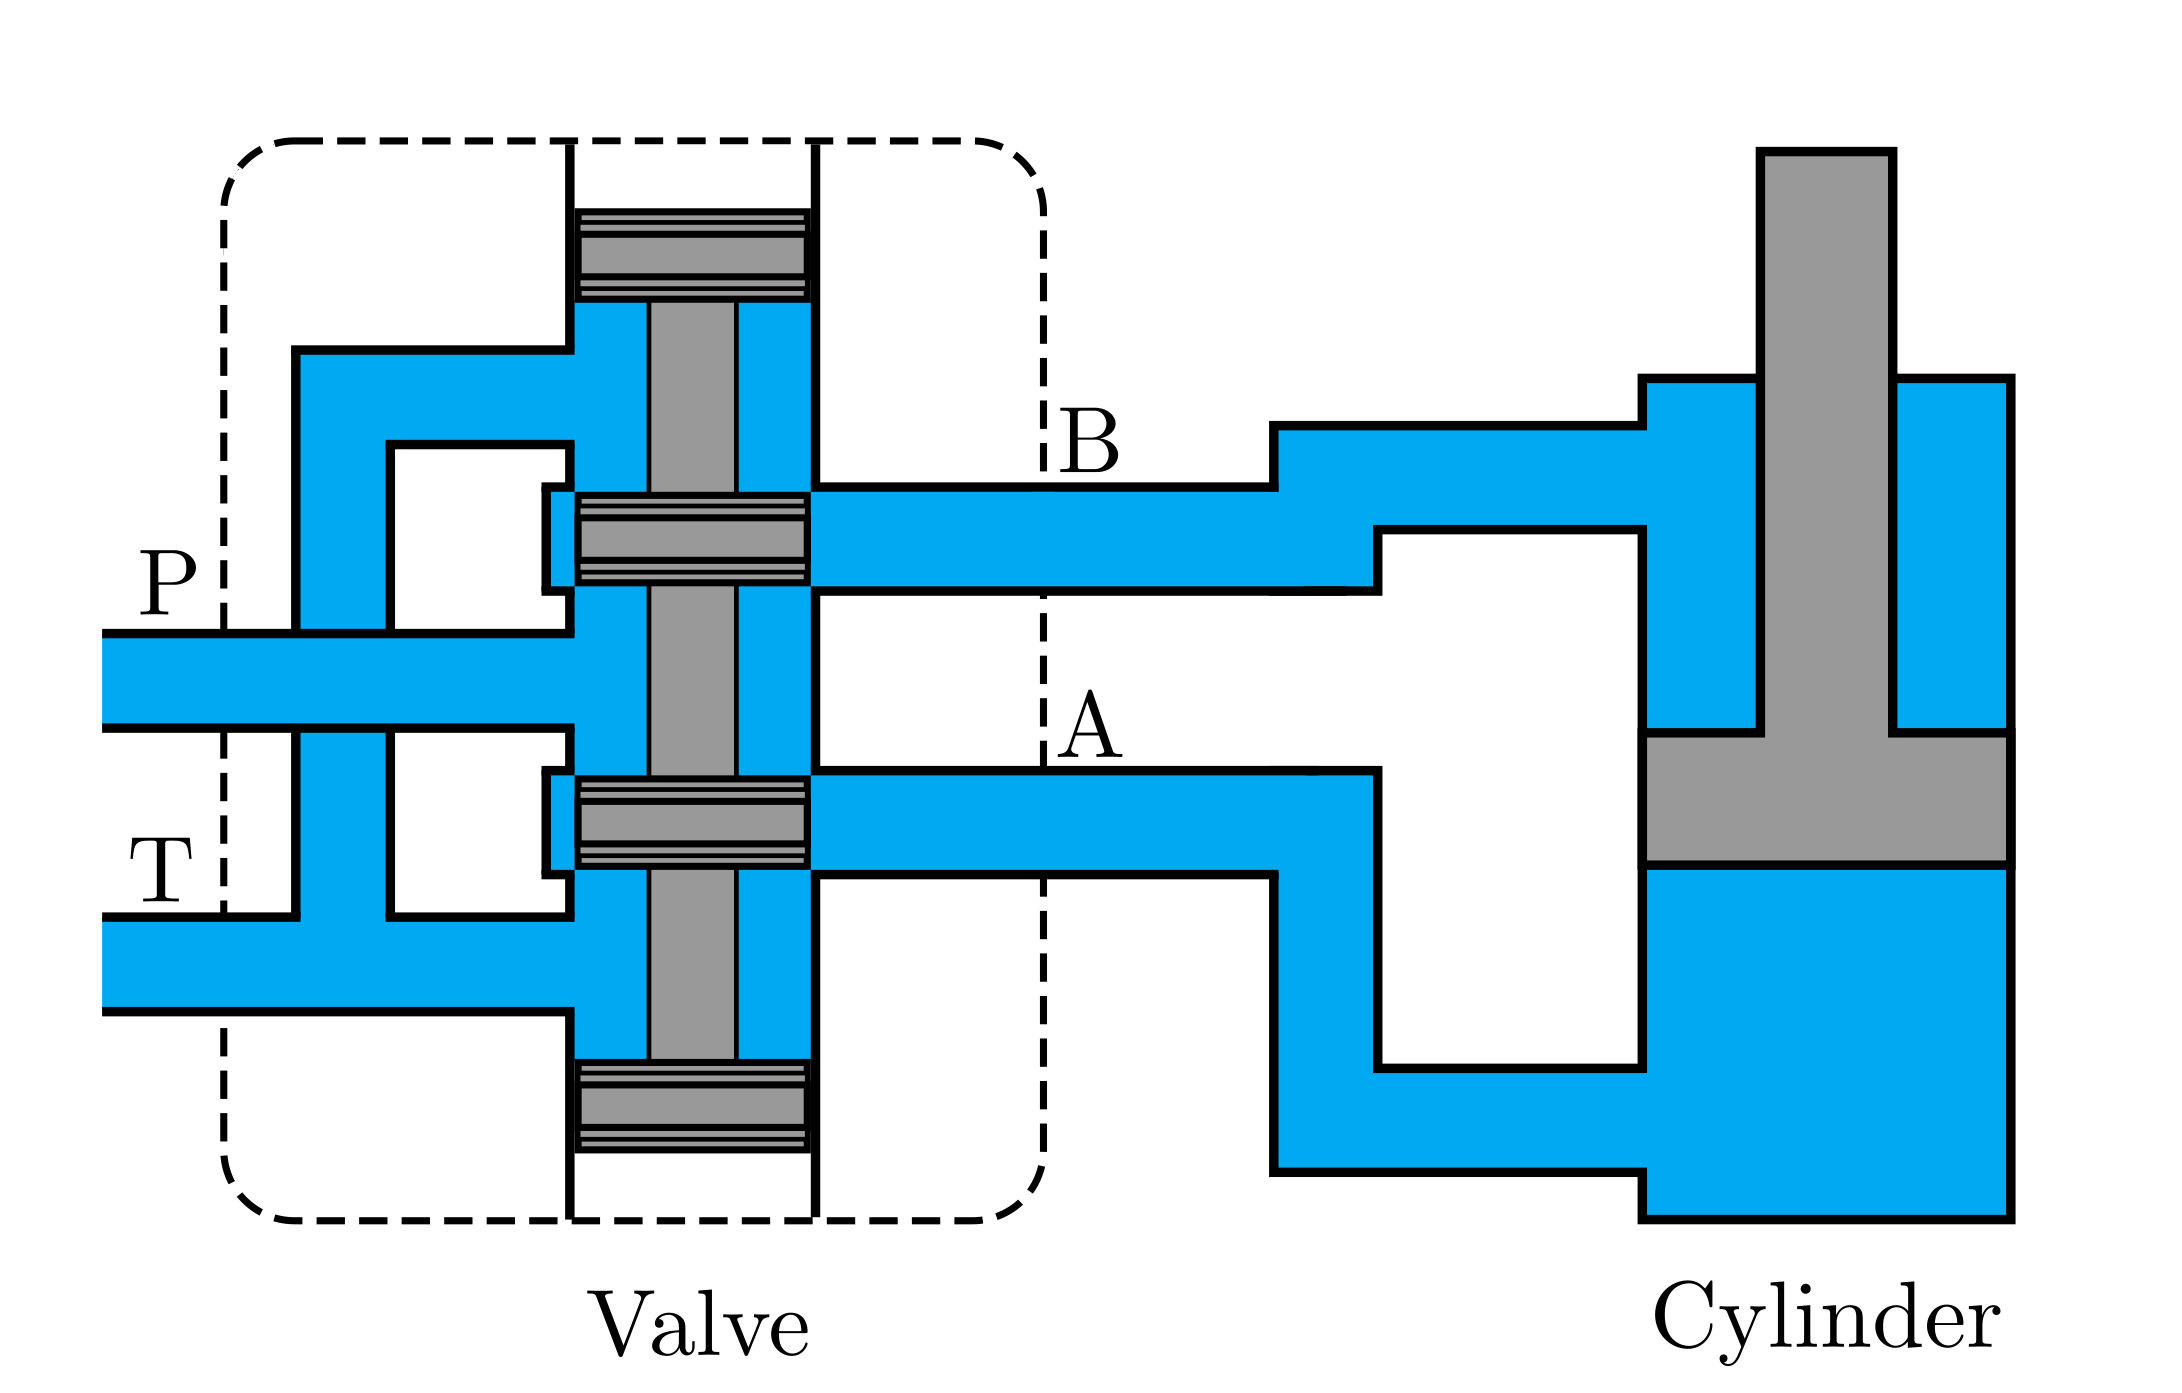
\includegraphics[keepaspectratio, scale=1.0]{contents/基礎方程式/figure/valve-cylinder.png}
        \caption{サーボバルブの図}
        \label{fig:figlabel}
\end{figure}

\section{サーボバルブ}
\subsection{サーボバルブの各部名称とパラメータ}
ここでは4ポート式サーボバルブの各部名称,および変数設定について述べる.
\begin{figure}[t]
    \centering
        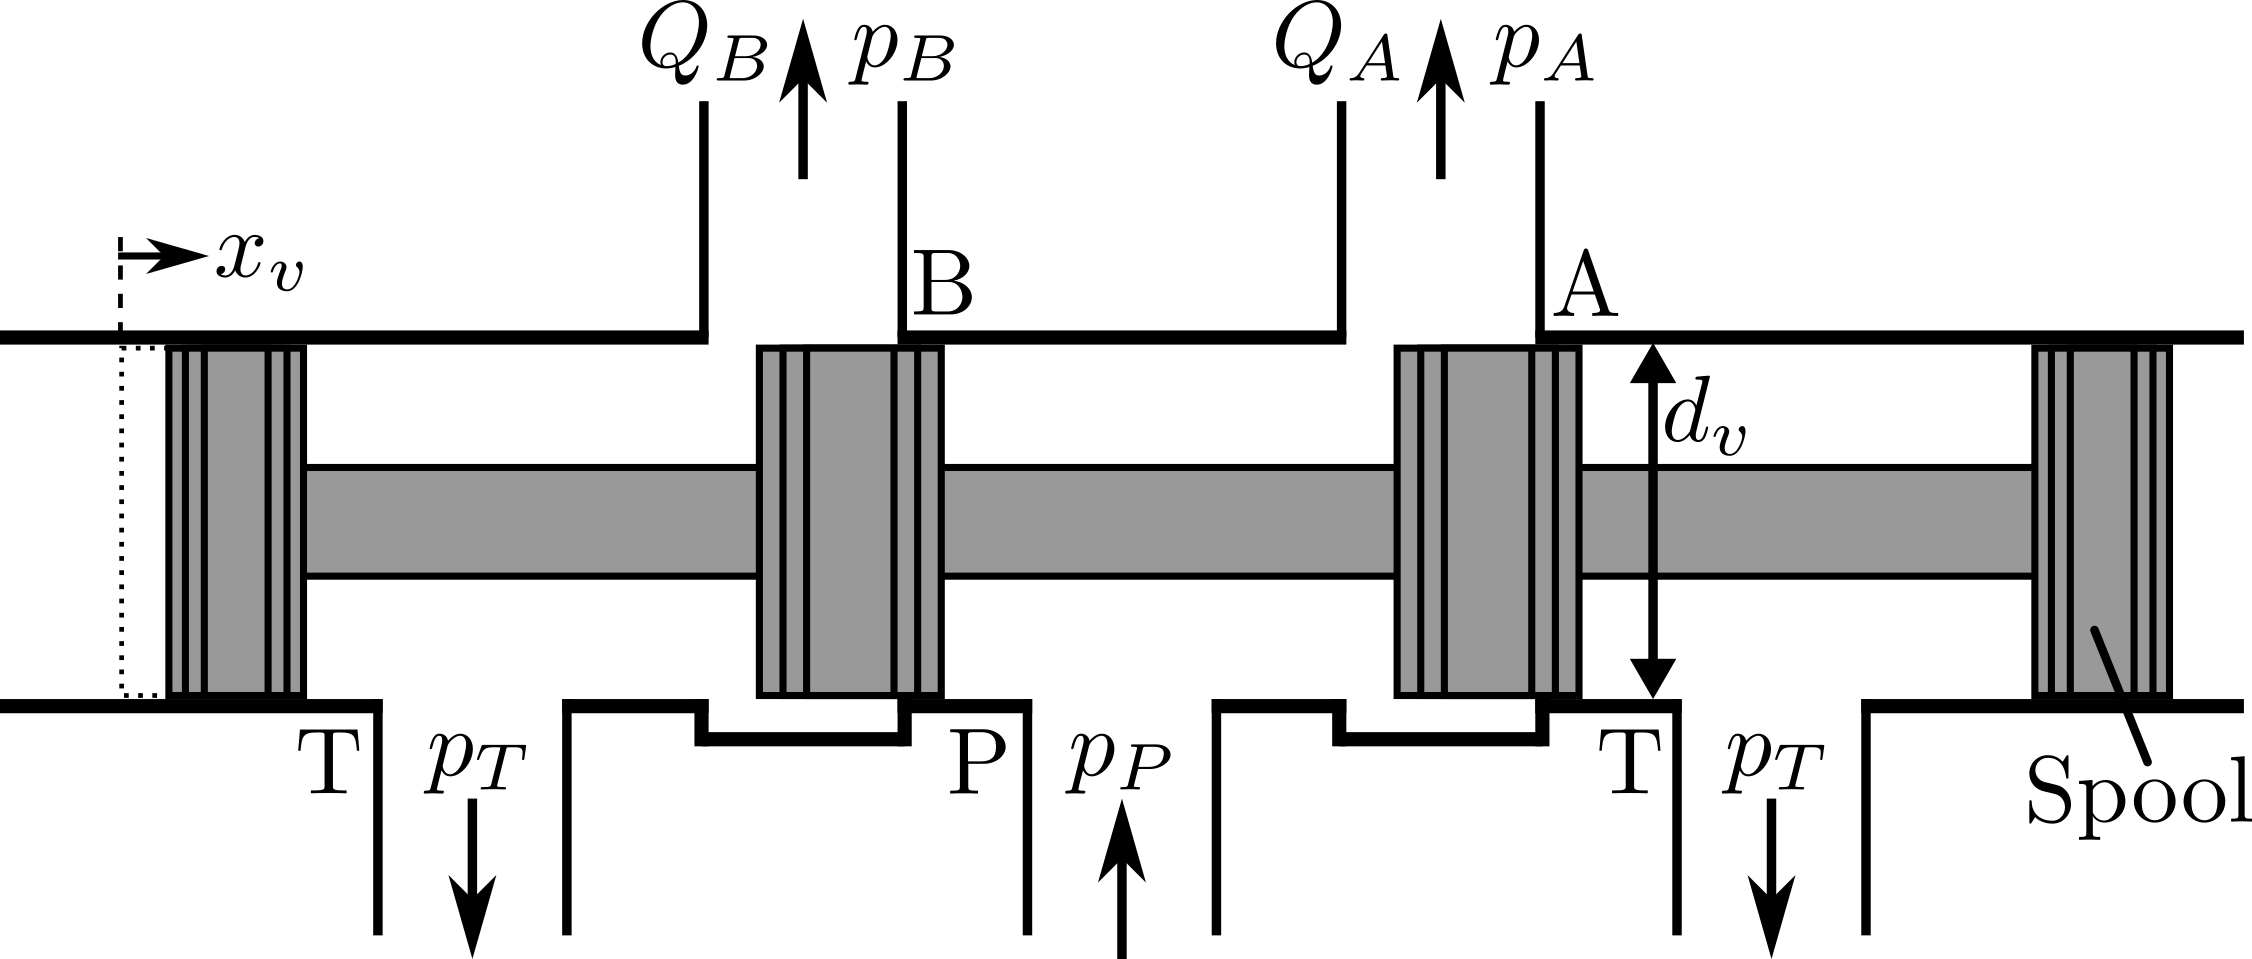
\includegraphics[keepaspectratio, scale=1.0]{contents/基礎方程式/figure/valve.png}
        \caption{サーボバルブの図}
        \label{fig:figlabel}
\end{figure}
\subsection{サーボバルブを通過する流量}
作動流体がサーボバルブを通過する流れは,オリフィス流れであるとみなされる.
オリフィスを通過する流量$Q$は,一般に
\begin{equation}
    Q = \alpha_d A \sqrt{\frac{2}{\rho}\Delta p}
    \label{eq:orifice_flow}
\end{equation}
と表される.
ここで,$\alpha_d$は流出係数(discharge coefficient),$A$は流体の断面積,$\rho$は流体の密度,$\Delta p$はオリフィス前後の十分離れた場所における流体の圧力の差である.
サーボバルブにおけるスプールの中立点からの変位を$x_v$とし,流体の流れる方向を考慮すると,\eqnname\ref{eq:orifice_flow}は
\begin{align}
    \label{eq:orifice_valve}
    Q(x_v,\Delta p)&= c_vx_v\mathrm{sign}(\Delta p)\sqrt{\Delta p}\\
    c_v &= \pi d_v \alpha_d\sqrt{\frac{2}{\rho}}
\end{align}
となる.
$\mathrm{sign}(\cdot)$はシグナム関数であり,以下で定義される.
\begin{align}
    \label{eq:function_sign}
    \mathrm{sign}(x) = 
    \begin{cases}
        1~&(\mathrm{if}~x>0)\\
        0~&(\mathrm{if}~x=0)\\
        -1~&(\mathrm{if}~x<0)
    \end{cases}
\end{align}

サーボバルブの制御ポートAから吐き出される流量$Q_A$は,「供給ポートPから制御ポートAへ流れる流量$Q_{PA}$」と「制御ポートAから戻りポートTへの流量$Q_{AT}$」の差分で表される.
供給ポートPから制御ポートAへ流れるときのスプール変位$x_v$を正とすると,このときには$Q_{AT}$は0となる.
逆に$x_v$が負のときには$Q_{PA}$は0となる.
これらをまとめると,$Q_A$は,\eqnname\ref{eq:orifice_valve}も考慮すると,
\begin{align}
    \notag
    \label{eq:flow_QA}
    Q_A =& Q_{PA}- Q_{AT} \\ \notag
    =&c_{v_{PA}}\mathrm{sg}(x_v)\mathrm{sign}(p_P-p_A)\sqrt{|p_P-p_A|} \\ 
    &- c_{v_{AT}}\mathrm{sg}(-x_v)\mathrm{sign}(p_A-p_T)\sqrt{|p_A-p_T|}
\end{align}
となる.
同様に,制御ポートBへ吐き出される流量$Q_B$は,向きが$Q_A$と逆になることに注意して
\begin{align}
    \label{eq:flow_QB}
    \notag
    Q_B =& Q_{PB}- Q_{BT} \\ \notag
    =&-c_{v_{PB}}\mathrm{sg}(-x_v)\mathrm{sign}(p_P-p_B)\sqrt{|p_P-p_B|} \\ 
    &+ c_{v_{BT}}\mathrm{sg}(x_v)\mathrm{sign}(p_B-p_T)\sqrt{|p_B-p_T|}
\end{align}
となる.
$\mathrm{sg}(\cdot)$は,
\begin{align}
    \label{eq:function_sg}
    \mathrm{sg}(x) = 
    \begin{cases}
        x&(\mathrm{if}~x>0)\\
        0&(\mathrm{if}~x\leq0)\\
    \end{cases}
\end{align}
で定義される関数である.

\subsection{サーボバルブの動特性}
サーボバルブへの指令電圧入力$u_v$とスプール変位$x_v$の関係は,周波数応答などから\eqnname\ref{eq:valve_freq}に示す二次系の運動方程式で近似して表すことができる.
\begin{equation}
    \label{eq:valve_freq}
    \frac{1}{\omega_v^2}\ddot{x}_v^* + \frac{2D_v}{\omega_v}\dot{x}_v^* + x_v^* + f_{hs}\mathrm{sign}(\dot{x}_v^*) = K_v u_v^*
\end{equation}
なお,$u_v^*$や$x_v^*$などはそれぞれ入力電圧の最大値$u_{v,max}$,スプール変位の最大値$x_{v,max}$で除して正規化されたものであり,以下の\eqnname\ref{eq:normalize_u}から\eqnname\ref{eq:normalize_xv}で定義される.
\begin{align}
    \label{eq:normalize_u}
    u_v^* &= \frac{u_v}{u_{v,max}}\\
    \label{eq:normalize_xv}
    x_v^* = \frac{x_v}{x_{v,max}}~,~\dot{x}_v^* &= \frac{\dot{x}_v}{x_{v,max}}~,~\ddot{x}_v^* = \frac{\ddot{x}_v}{x_{v,max}}
\end{align}
また,\eqnname\ref{eq:valve_freq}において$K_v$はバルブのゲイン,$\omega_v$は固有角振動数,$D_v$は粘性係数,$f_{hs}$はバルブのヒステリシスや応答感度を表す関数である.

\section{油圧シリンダー}
油圧シリンダー内の作動流体についてモデル化する.
流体の質量保存則は\eqnname\ref{eq:situryouhozon}である.
\begin{equation}
    \label{eq:situryouhozon}
\Sigma \dot{m}_{\mathrm{in}}-\Sigma \dot{m}_{\mathrm{out}} = \frac{\mathrm{d}(\rho V)}{\mathrm{d}t} = \rho \dot{V}+\dot{\rho}V
\end{equation}
$\rho$は流体の密度であり,圧縮性流体においてはその表現方法は文献により様々であるが,本論文では以下の\eqnname\ref{eq:rho_teigi}で定義される$\rho$を採用する.
\begin{equation}
    \label{eq:rho_teigi}
    \rho = \rho_i + \frac{\rho_i}{E(p)}p
\end{equation}
ここで$\rho_i$は圧力が0のときの密度,$E(p)$はバルクモジュールである,$p$は流体の圧力である.
\eqnname\ref{eq:situryouhozon}と\eqnname\ref{eq:rho_teigi}より
\begin{equation}
    \label{eq:流量保存}
    \Sigma Q_{\mathrm{in}} - \Sigma Q_{\mathrm{out}} = \dot{V} + \frac{V}{E(p)}\dot{p}
\end{equation}
となる.
よって,シリンダ内の流量は次の\eqnname\ref{eq:シリンダ内流量(rod)}および\eqnname\ref{eq:シリンダ内流量(head)}で表される.
\begin{align}
    \label{eq:シリンダ内流量(rod)}
    Q_{\mathrm{rod}}& = \dot{V}_\mathrm{rod} + \frac{V_\mathrm{rod}}{E(p_\mathrm{rod})}\dot{p}_\mathrm{rod}\\
    \label{eq:シリンダ内流量(head)}
    Q_{\mathrm{head}} &= \dot{V}_\mathrm{head} + \frac{V_\mathrm{head}}{E(p_\mathrm{head})}\dot{p}_\mathrm{head}
\end{align}
\section{モデルの線形化とラプラス変換}

\section{運動方程式と摩擦のモデル}
%\chapter{システムの線形性とその同定}
前章で導出した物理モデルにはバルクや粘性項などのパラメータが含まれている.
これらのパラメータを全て知ることができればシリンダのモデルを得ることが可能であるが,現実的に組み合わせることは難しい.
そこで本章ではシステム同定を用いて油圧システムのモデルの構築を行う.
バルブへの電圧入力からシリンダ先端の位置及び先端で発生する力までのモデルを,システム同定を用いて導出する.
力の同定ではシリンダ先端を固定した状態で同定をする.
位置の同定にあたっては無負荷状態で行う.
%同定にあたってはシステムの周波数応答を調べて特徴を把握したのちに最小自乗法によるモデルの同定,およびM系列を用いた同定を行いそれぞれを比較する.
\section{実験機とその構成}
本研究で使用する油圧システムの実験装置を\figname\ref{fig:}に示す.
本装置は片ロッドの油圧シリンダ,ギヤポンプ,サーボバルブなどにより構成されており,シリンダにはワイヤー式エンコーダとロードセルが取り付けてある.
また,圧力センサをサーボバルブのAポートおよびBポート,そしてシリンダのヘッド側とロッド側の入り口の計4箇所に取り付けてある.
本装置に用いている各部品の諸元をTable~\ref{tab:}にまとめる.

\begin{table}[t]
    \begin{tabular}{|c|c|}
        hoge & hoge\\
        hoge & hoge
    \end{tabular}
\end{table}


\section{先端で発生する力までの線形性とモデルの同定}
\subsection{線形性調査}
\subsection{周波数応答}
\subsection{最小自乗法による伝達関数モデルの同定}
\section{位置までの同定}
\subsection{線形性調査}
\subsection{周波数応答}
\section{M系列による同定}
\subsection{M系列の性質}
\subsection{システム同定(入力から位置)}
\subsection{システム同定(入力から力)}


%\chapter{力制御}
この章は力制御について書く
力制御のgitどこにいった
%\chapter{切り替え制御}
%\chapter{結言}
本論文では,6軸油圧マニピュレータの力制御に向けて,油圧シリンダを用いた力推定手法の構築および力制御を行った.
力推定にはシステム同定の手法を活用して得た油圧システムのモデルを利用し,制御においてはPID制御やI-PD生制御,$H_\infty$制御の適用を行った.
そしてこれらを位置制御と組み合わせ,コンプライアンス制御においてはフィードバック変調器(FBM)を用いることで摩擦補償を行う手法の提案を行った.

得られた主な結果を以下に示す.
\begin{itemize}
    \item 力推定において,シリンダ推力$\fthr$から実測出力$\fmsr$までの伝達関数$\GfthrTofmsr$を同定することにより,圧力センサを用いた力推定を行った.そしてモデルの同定にはむだ時間の考慮が必要であるとの知見を得た.
    \item バルブへの指令電圧から位置までのシステム同定においては,積分器を含むことを陽に考慮して同定を行うことで,より良い同定結果が得られることを示した.
    \item 力制御においては,$H_\infty$制御の適用により,外乱抑制の効果があることを確かめた.
    \item コンプライアンス制御において,フィードバック変調器を用いることで,積分器を利用せずとも定常応答の改善ができることを実験により示した.
\end{itemize}

今後は6軸油圧マニピュレータに力制御を適用し,ならい制御などを実現していくことが目標である.

% \input{./contents/1_introduction/1_introduction.tex} %第1章
% \input{./contents/2_how_to_write/2_how_to_write.tex} %第2章
% \input{./contents/3_latex_knowhow/3_latex_knowhow.tex} %第3章
% \input{./contents/4_end/4_end.tex} %第4章

% \input{./contents/9_bibliography/9_bibliography.tex} %参考文献

%付録
\appendix
% \input{./contents/A_eom/A_eom.tex} %付録A

%
%後書き
\backmatter
%謝辞
%\input{./contents/Z_thanks/Z_thanks.tex}


\end{document}
